
\subsection{Task scheduling}
Consider a cloud service that offers distributed infrastructure to process
jobs, or a modern data processing system that processes queries on large
databases.
In such systems, queries may be passed to an execution planner
which uses statistics, current workloads, and cost models to choose an optimal
plan among a set of candidate execution plans.
These plans are in the form of directed acyclic graphs with edges indicating
task dependencies.
Some metrics for choosing plans include makespan (time to finish executing
the DAG) and resource consumption (e.g., to obtain fairness between queries).
One challenge, however, is that available resources change with time,
so an execution plan deemed optimal before execution can become sub-optimal
during its lifetime~\cite{mahajan2018qoop}.

With this as setting, one may consider learning a decision rule for
scheduling tasks.
We consider $\X$ to be some set of feature vectors
(extracted from the query, tasks, resources at time of execution,
time-of-day, and so on), and $\Y$ to be the set of preference graphs with
appropriate augmentation depending on the metric of interest. Samples
$S = \{((x_{i,j})_{j=1}^{n_i}, y_i)_{i=1}^m\}$ may come from computing the best DAG
in hindsight and collecting statistics. We want the learning algorithm to
output a DAG that minimizes $\ell$-risk for some suitable loss $\ell$.

If we make the simplification that execution of plans proceed in rounds (e.g.\
MapReduce), ranking techniques can be brought to bear. Specifically,
let the prediction space be
$\Yh = \{f: \bigcup_{i=1}^n \X^n \to \mathbb{Z}_+\}$,
i.e.\ functions which stratifies jobs into rounds. This is no different from
functions that output relevance scores.

\subsubsection{Minimizing Job Completion Time and Parallel Processing Cost?}
Here, we want the scoring function to output as few rounds as possible.
A way to do this is as follows. For $r$ items, let
\begin{align*}
  \Y_r &= \{ (G, \vec{c})
  \mid \text{$G$ is a weighted DAG on $[r]$ and $\vec{c} =( c_1, \ldots, c_r), c_1< ...< c_r$}
  \}.
\end{align*}
The label space is $\Y = \Y_r$ is a set of finite number of weighted DAGs
over $r$ items. We interpret each $c_i$
to be the unit cost incurred for scheduling a task past round $i$.
The prediction space $\mathcal{T}$ has size $r^r$

The loss $\ell$ can then be defined as:
\begin{align*}
  \ell(f, (G, \vec{c}))
  = \sum_{i,j: i \neq j} w_{i,j}^G \1_{f(i) \geq f(j)}
  + \sum_{i=1}^n c_i \sum_{j=1}^n \1_{f(j) \geq i}
\end{align*}


\textcolor{red}{Mingyang: The loss defined below eq(1) is easier to analyze and have the same property to penalize depth.}


%%%%%%%%%%%%%%%%%%%%%%%%%%%%%%%
\subsubsection{Mingyang's draft for Minimizing Job Completion Time}

TODO:
\begin{itemize}
\item Nicolas: Explanation of the problem, possibility of using ranking
  algorithms to solve this problem. 
\item Shivani's method that justifies using squared loss as a surrogate
  (justification: it is consistent). This reduces the problem to just a
  clustering problem giving a ranking.
\item Connection between surrogate score output $u_{ij}$'s and the analysis
  of the expected graph. Clarifying notation that $y_{ij} = \E_G[y_{ij}]$.
\item Preliminary result: Under some assumptions on the distribution of graphs,
  the Bayes-consistent clustering must respect the Bayes-consistent ranking.
\item Change $m$ to $\sigma^*$ in Assumption.
\item Strengthen clusters to adjacent clusters in proof. 
\item Using uniqueness condition in proof. 
\end{itemize}

\iffalse
Let consider $5$ items. The true permutation $\sigma^*: \sigma^*(i)=i$. If we have a mapping $m$ with $m(1)=1, m(2,4)=2, m(3,5)=3$, then it has a wrong ranking for pair $(3,4)$. Let $m'$ be the flip mapping. 
\begin{itemize}
	\item $l(m)=y_{24}+y_{42}+y_{35}+y_{53}+y_{34}$
	\item $l(m')=y_{23}+y_{32}+y_{45}+y_{54}$
\end{itemize}
If $y_{34}=1, y_{43}=0$, which is the only edge in the difference, and $y_{24}=y_{42}=0,y_{35}=y_{53}=0$, $y_{23}=y_{32}=1, y_{45}=y_{54}=0$. Then $l(m)=1<l(m')=2$
\fi


\begin{equation}\label{eq:pdloss}
\begin{split}
%\text{Target Loss: }l: \mathcal{Y}\times\mathcal{T}, \text{ with } l((\mathbf{y},\mathbf{c}),  m)=\sum\limits_{i\not=j}y_{ij}1_{\{m(i)\geq m(j)\}}+\sum\limits_{i=1}^rc_i\big(\sum_{j=1}^r1_{\{m(j)\geq i\}}\big)=(\mathbf{y}', \mathbf{c}')\begin{pmatrix} \mathbf{\Phi}_1(m) \\\mathbf{\Phi}_2(m) \\\end{pmatrix} 
\text{Target Loss: }l: \mathcal{Y}\times\mathcal{T}, \text{ with } l((\mathbf{y},\mathbf{c}),  m)=\sum\limits_{i\not=j}y_{ij}1_{\{m(i)\geq m(j)\}}+\sum\limits_{i=1}^rc_i1_{\{(\max_jm(j))\geq i\}}=(\mathbf{y}', \mathbf{c}')\begin{pmatrix} \mathbf{\Phi}_1(m) \\\mathbf{\Phi}_2(m) \\\end{pmatrix} 
\end{split}
\end{equation}
, where $\mathbf{\Phi}_1(m)$ is $r(r-1)$ length vector with entries $1_{\{m(i)\geq m(j)\}}$, and  $\mathbf{\Phi}_2(m)$ is $r$ length vector with entries $1_{\{(\max_jm(j))\geq i\}}$.  By Theorem 3 \cite{ramaswamy2013convex}, we have $l$-calibrated surrogate $(\psi_l^*, \text{pred}_l^*)$ , where
\begin{equation*}
\begin{split}
\psi_l^*((\mathbf{y},\mathbf{c}), (\mathbf{u}, \mathbf{v}))=\sum\limits_{i\not=j}^{r}(u_{ij}-y_{ij})^2+\sum\limits_{k=1}^r(v_k-c_i)^2,\quad \text{pred}_l^*(\mathbf{u}, \mathbf{v})\in\text{argmin}_{m\in \mathcal{T}}\bigg(\mathbf{u}'\mathbf{\Phi}_1(m)+\mathbf{v}'\mathbf{\Phi}_2(m)\bigg)
\end{split}
\end{equation*}
It is easy to see that solving $\text{pred}_l^*$ is same as solving original PD-loss problem. 



Let $m^*: [r]\rightarrow [r]$ be the optimal solution of eq(\ref{eq:pdloss}), and let $|m|=\max_jm(j)$. We notice that $m$ must satisfies the below two rules.
\begin{lemma}
	Fact1(no gap): For any $k\in[|m|]$, $m^{-1}(k)\not=\emptyset$. 
\end{lemma}
\begin{proof}
If there exists such a $k$, then we can move all the items ranked lower than $k$ w.r.t $m$ by one level, i.e, set $m'(l)=m(l)-1, \forall l, m(l)>k$. We can reduce the target loss by $c_{|m|}>0$, which contradicts that $m$ is optimal.
\end{proof}

Before deriving the second fact, we first re-examine the target loss. The target loss can be written as three parts: pdloss, clusterloss, depthloss$$\sum\limits_{i\not=j}y_{ij}1_{\{m(i)> m(j)\}}+\sum\limits_{i\not=j}y_{ij}1_{\{m(i)= m(j)\}}+\sum\limits_{i=1}^rc_i1_{\{(\max_jm(j))\geq i\}}$$

\begin{assumption}
	There is a unique total order $\sigma^*$. For any  $i\not=j $, wlog $m(i)<m(j)$
	$$y_{ij}+y_{ji}\geq \sum\limits_{k\in \{l: \sigma^*(l)\in [m(i), m(j)]\}, l={(\sigma^*)}^{-1}(\sigma^*(k)+1)\}}y_{kl}+y_{lk}$$
\end{assumption}
It means under total ranking, clustering two nodes will incur strict bigger loss than sum of  clustering loss of any two items between them. 

\begin{lemma}
Fact2(respect DAG): If $\sigma^*(k)<\sigma^*(l)$, then $m(k)\leq m(l)$.
\end{lemma}
\begin{proof}
	If not, then for $m$, there must exist two clusters which do not respect DAG. That is to say, for some $k<l$, and let the first cluster $C_1=\{i: m(i)=k\}$, the second $C_2=\{j:m(j)=l\}$, $\exists \text{ pair } (i,j)\in (C_1, C_2)$, $\sigma^*(i)>\sigma^*(j)$. Now consider $m'$ which flip all these pairs of $m$ until we can not find more such pairs. and keep the rest of clusters unchanged. When we cannot find more such pairs, let $C_{1,u}$ be items previously in $C_1$ and now still in $C_1$;   $C_{1, d}$ be items previously in $C_1$ but now in $C_2$;  et $C_{2,u}$ be items previously in $C_2$ but now in $C_1$;   $C_{2, d}$ be items previously in $C_2$ and now still in $C_2$. Since we only do flip pairs, $|C_{1,d}|=|C_{2,u}|$.
	\begin{equation}
	\begin{split}
	&C_1=  C_{1,u}\cup C_{1,d}\\
		&C_2=  C_{2,u}\cup C_{2,d}\\
		&m: m(C_1)=k; m(C_2)=l\\
		&m': m'(C_{1, u}\cup C_{2, u})=k; m'(C_{1,d}\cup C_{2, d})=l\\
	\end{split}
	\end{equation}
	\begin{itemize}
		\item pdloss: $m'$ will have no greater pdloss than $m$, because $m'$ respect more ranking than $m$.
		\item depthloss: $m$ and $m'$ have same depthloss.
		\item clusteringloss: let $C_{cl}(m)$, $C_{cl}(m')$ be clusteringloss for $m, m'$
		\begin{itemize}
			\item $C_{cl}(m)=\bigg(\sum\limits_{i\in C_{1, u}, j\in C_{1, u}}y_{ij} + \sum\limits_{i\in C_{2, d}, j\in C_{2, d}}y_{ij} \bigg)+ \bigg(\sum\limits_{i\in C_{1, u}, j\in C_{1, d}}(y_{ij}+y_{ji}) \bigg)+\bigg( \sum\limits_{i\in C_{2, u}, j\in C_{2, d}}(y_{ij}+y_{ij})\bigg)$
						\item $C_{cl}(m')=\bigg(\sum\limits_{i\in C_{1, u}, j\in C_{1, u}}y_{ij} + \sum\limits_{i\in C_{2, d}, j\in C_{2, d}}y_{ij} \bigg)+ \bigg(\sum\limits_{i\in C_{1, u}, j\in C_{2, u}}(y_{ij}+ y_{ij})\bigg)+\bigg( \sum\limits_{i\in C_{1, d}, j\in C_{2, d}}(y_{ij}+y_{ij})\bigg)$
		\end{itemize}
	By our flip rule, $\sigma^*(i)>\sigma^*(j)$ for any $i\in C_{1,d}\cup C_{2,d}, j\in C_{2,u}\cup C_{1,u}$. If not, the fliping process will not stop. Since the first big bracket is same for $m$ and $m'$, we only work on the rest two. For any $i\in C_{1,u}$, $j\in C_{2,d}, k\in C_{2,u}, l\in C_{1,d} $, There are four possibilities:
	\begin{itemize}
		\item $\sigma^*(k)<\sigma^*(i)<\sigma^*(j)<\sigma^*(l)$
			\item $\sigma^*(k)<\sigma^*(i)<\sigma^*(l)<\sigma^*(j)$
				\item $\sigma^*(i)<\sigma^*(k)<\sigma^*(j)<\sigma^*(l)$
					\item $\sigma^*(i)<\sigma^*(k)<\sigma^*(l)<\sigma^*(j)$
	\end{itemize}
For the first case
\begin{equation*}
\begin{split}
(y_{il}+y_{li})+(y_{kj}+y_{jk})&\geq (y_{ij}+y_{ji}+y_{jl}+y_{li}) + (y_{ki}+y_{ik}+y_{ij}+y_{ji})\\
&>y_{ik}+y_{ki}+y_{jl}+y_{lj}\\
\end{split}
\end{equation*}
For the second case
\begin{equation*}
\begin{split}
(y_{il}+y_{li})+(y_{kj}+y_{jk})&\geq (y_{il}+y_{li}) + (y_{ki}+y_{ik}+y_{ij}+y_{ji}+y_{lj}+y_{jl})\\
&>y_{ik}+y_{ki}+y_{jl}+y_{lj}\\
\end{split}
\end{equation*}
For the third case
\begin{equation*}
\begin{split}
(y_{il}+y_{li})+(y_{kj}+y_{jk})&\geq(y_{kj}+y_{jk}) + (y_{ki}+y_{ik}+y_{kj}+y_{jk}+y_{lj}+y_{jl})\\
&>y_{ik}+y_{ki}+y_{jl}+y_{lj}\\
\end{split}
\end{equation*}
For the fourth case
\begin{equation*}
\begin{split}
(y_{il}+y_{li})+(y_{kj}+y_{jk})&\geq (y_{kl}+y_{lk}+y_{jl}+y_{li}) + (y_{ki}+y_{ik}+y_{kl}+y_{lk})\\
&>y_{ik}+y_{ki}+y_{jl}+y_{lj}\\
\end{split}
\end{equation*}
	\end{itemize}

Note that the above inequality is from unique ordering and low.noise condition, because for any $(i,j)$, wlog $m(i)<m(j)$, then $y_{ij}>y_{ji}\geq 0$, which implies $y_{ij}+y_{ji}>0$. Above calculation shows $C_{cl}(m)>C_{cl}(m')$ which contradicts optimality of $m$.
	
\end{proof}



\begin{lemma}
	The optimal $m^*\in\mathcal{M}$, where  $\mathcal{M}$ is a set containing all elements satisfying Fact2.
\end{lemma}


\begin{comment}
Note that if there is a \underline{unique} total order $\sigma^*$, then $\mathcal{M}=\{\sigma^*\}$, and $m$ can be derived by clustering items in $m^*_{pd}$. This motivates us a naive algorithm for deriving $m^*$. Basically, we start from $\sigma^*$, and find the best way to cluster items, that is, reduce the target loss by 
$$\textbf{ Increase SMALL loss (from $\mathbf{y}$)by clustering, but decrease BIG loss (from $\mathbf{c}$) by smaller depth }$$

We also notice that minimizing eq(\ref{eq:pdloss}) is equivalent to minimize the following quantity:
	\begin{equation*}
	\text{argmin}_ml((\mathbf{y},\mathbf{c}),  m)= \text{argmin}_m\sum\limits_{i=1}^r\sum\limits_{j=1}^{i-1}(y_{ij}-y_{ji})1_{\{m(i)> m(j)\}}+\sum\limits_{i=1}^r\sum\limits_{j=1}^{i-1}y_{ij}1_{\{m(i)= m(j)\}}+\sum\limits_{i=1}^rc_i1_{\{(\max_jm(j))\geq i\}}\\
	\end{equation*} 

Before we present first algorithm, we start from some notations. For any $m\in \mathcal{M}$, by fact1, we know $m^{-1}(i)\not=\emptyset$ for $i\leq |m|$. 
\begin{itemize}
	\item Let $\mathcal{C}^m=\{  \{m^{-1}(i)\}_{i=1}^{|m|}     \}$ be set of clusters of $m$
	\begin{itemize}
		\item $\mathcal{C}^m[i]= \{m^{-1}(i)\}$ is set of items in cluster $i$ under $m$
		\item Note that $\sigma^*$ has $r$ clusters, and each has one  and only one item.
	\end{itemize}
\item Let cost of merging cluster $i$ and $i+1$ under $m$ be \begin{equation}\label{eq:cost}
\begin{split}
cost^m_{i, i+1}&=\sum\limits_{n_1\in \mathcal{C}^m[i]}\sum\limits_{n_2\in \mathcal{C}^m[i+1]}\bigg(-(y_{n_1n_2}^\mathbf{p}-y_{n_2n_1}^\mathbf{p})1_{n_1>n_2}1_{\{m(n_1)> m(n_2)\}}+y_{n_1n_2}^\mathbf{p}1_{n_1>n_2}+y_{n_2n_1}^\mathbf{p}1_{n_2>n_1}\bigg)\\
\end{split}
\end{equation}
, where each summand is non-negative.
\end{itemize}

	We first derive a consistent permutation $\sigma^*$ under low.noise condition(or related conditions) \cite{ramaswamy2013convex}, \cite{duchi2010ranking}, and then plug $\sigma^*$ into below algorithm. If there is a unique total ranking and it satisfies low.noise assumptions, we will find a $m$ achieving lowest target loss.
	
	\begin{lemma}
	Given $m$,  define $cost=\text{min}_{i\in [|m|-1]} cost^m_{i, i+1}$. $cost$ is non-decreasing after each clustering.
	\end{lemma}
\begin{proof}
	Consider we have $m$, and then we cluster $i, i+1$ to have $m'$. We need to show $\text{min}_{l\in [|m|-1]} cost^m_{l, l+1}\leq \text{min}_{l'\in [|m'|-1]} cost^{m'}_{l', l'+1}$. Notice that $cost^m_{l, l+1}=cost^{m'}_{l', l'+1}$ for $l=l'+1$ and $l\not= i, i+1$. Also $cost^m_{i-1, i}\leq cost^{m'}_{i-1, i}$ because now there are more items in $i$-th cluster under $m'$ and each summand  of eq(\ref{eq:cost}) is non-negative. Same reason for $cost^m_{i, i+1}\leq cost^{m'}_{i, i+1}$. 
	\end{proof}
Thanks to the fact that $c_i$ is strictly increasing, this lemma implies once $c_{cur}-cost$ is negative, any kind of clustering in the future will increase target loss. This justifies the stopping condition in the algorithm. 

\begin{algorithm}[H]
	\caption{Naive algorithm}
	\begin{algorithmic}[1]
		\Procedure{Clustering ranking }{$\mathcal{G}, \mathbf{p}, \mathbf{c}, \sigma$}
		\State Initialize $cur=r$
		\For{\texttt{$i\in[r-1]$}}
		\State
		Let $cost=\text{min}_{i\in [|m|-1]} cost^m_{i, i+1}$
		\State 
		Let $cl = \text{argmin}_{i\in [|m|-1]} cost^m_{i, i+1}$
		\If{$cost\leq c_{cur}$}
		\State Merge clusters $cl$ and $cl+1$. That is, 
		set $m^{-1}(cl)\leftarrow m^{-1}(cl)\cup m^{-1}(cl+1)$; set $m^{-1}(cl+i)\leftarrow m^{-1}(cl+i+1)$ for $i\geq 1$; and set $|m|\leftarrow |m|-1$.
		\State $cur\leftarrow cur-1$
		\Else\quad
			break; 
		\EndIf		
		\EndFor
		\State \textbf{return} $m$
		\EndProcedure
	\end{algorithmic}
\end{algorithm}
The last thing we should worry is that when there are more than $1$ permutation achieve lowest pd loss. We should note that we may only derive one permutation from algorithm in \cite{ramaswamy2013convex}, so whether other unoutputed permutation will achieve lower target loss?  The answer is YES. Let's look at an example.
\begin{figure}[h]
	\begin{center}
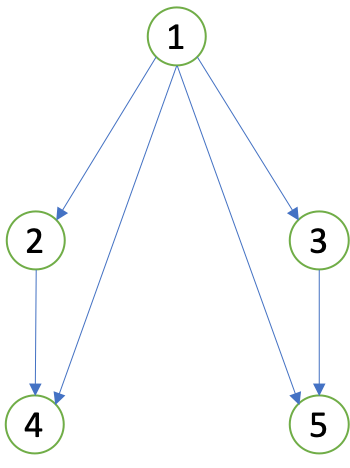
\includegraphics[scale=0.5]{figure/eg1.png}
	\end{center}
\end{figure}
The total ranking is not unique. $\sigma_1=(1,2,3,4,5)$ or $\sigma_2=(1,2,4,3,5)$ both minimize pd loss, but will have different solution in our case. Whether $\sigma_1$ or $\sigma_2$ got outputed depends on $(\mathcal{G}, \mathbf{p})$. If we utilize surrogates from Theorem 6 from \cite{ramaswamy2013convex}, 
\begin{equation*}
\begin{split}
u_2=-y_{12}^{\mathbf{p}}+y_{24}^{\mathbf{p}}\\
u_3 = -y_{13}^{\mathbf{p}}+y_{35}^{\mathbf{p}}\\
u_4 = -y_{24}^{\mathbf{p}}-y_{14}^{\mathbf{p}}\\
u_5 = -y_{35}^{\mathbf{p}}-y_{15}^{\mathbf{p}}\\
\end{split}
\end{equation*}
where according to the graph, $y_{21}^{\mathbf{p}}, y_{42}^{\mathbf{p}}, y_{41}^{\mathbf{p}}, y_{31}^{\mathbf{p}}, y_{51}^{\mathbf{p}}, y_{53}^{\mathbf{p}}=0$. It is easily to see that
\begin{equation*}
\begin{split}
\{y_{12}=100, y_{24}^{\mathbf{p}}=100, y_{13}^{\mathbf{p}}=100, y_{35}^{\mathbf{p}}=99, y_{14}^{\mathbf{p}}=200, y_{15}^{\mathbf{p}}=300\}\Rightarrow \sigma_1\\
\{y_{12}=100, y_{24}^{\mathbf{p}}=100, y_{13}^{\mathbf{p}}=400, y_{35}^{\mathbf{p}}=99, y_{14}^{\mathbf{p}}=200, y_{15}^{\mathbf{p}}=499\}\Rightarrow \sigma_2
\end{split}
\end{equation*}

Although $\sigma_1, \sigma_2$ are equivalent w.r.t pdloss, it is not for our case. Let $c_1=0, c_2=c_3=c_4=c_5=1$. Then if we start from $\sigma_1$, the best $m_1=(1,\{2,3\}, \{4,5\})$ and from $\sigma_2$, the best $m_2=(1,2,\{3,4\}, 5)$. However $m_1$ have smaller target loss. 

To solve this issue, we must go through all possible total ordering. That is, if we have all topological sorting of difference graph, we can run Algorithm 1 on each of them to find out the lowest target loss. Thanks to Theorem 7 of \cite{ramaswamy2013convex}, we will have a calibrated surrogates which will also give us all possible total ordering.

\begin{algorithm}[H]
	\caption{Improved algorithm}
	\begin{algorithmic}[1]
		\Procedure{xxx }{$\mathcal{G}, \mathbf{p}, \mathbf{c}$}
		\State Get $\mathcal{M}$ from Algorithm $1$ from \cite{ramaswamy2013convex}
		\State Let $m^*=NULL$, $loss = \infty$
		\For{\texttt{$\sigma\in\mathcal{M}$}}
		\State
		Let $m=${Clustering ranking }{($\mathcal{G}, \mathbf{p}, \mathbf{c}, \sigma$)}, with $l$ be the corresponding loss.
		\If{\texttt{$l\leq loss$}}
		Set $m^*=m$
		\EndIf
		\EndFor
		\State \textbf{return} $m^*$
		\EndProcedure
	\end{algorithmic}
\end{algorithm}

Warning: this algorithm only works under the assumption that $\mathcal{M}$ is small. If $\mathcal{M}$ is huge, then it would be hard to solve the problem quickly. Consider a DAG over $r$ items($r$ is even), with edges $\{(i,i+1)\}_{i=1}^{r/2}\cup \{(i,i+1)\}_{r/2+1}^r$. Then $|\mathcal{M}|=(\frac{r}{2}+1)!$. 

\end{comment}








